\documentclass[14pt, a4paper]{extreport}

\usepackage[utf8]{inputenc}
\usepackage[T1,T2A]{fontenc}
\usepackage[russian]{babel}
\usepackage{geometry}
\geometry{left=30mm, right=15mm, top=20mm, bottom=20mm}

\usepackage{setspace}
\onehalfspacing

\usepackage{graphicx}
\usepackage{hyperref}
\usepackage{booktabs}
\usepackage{amsmath}
\usepackage{amssymb}
\usepackage{listings}
\usepackage{xcolor}
\usepackage{caption}
\usepackage{float}
\usepackage{titlesec}
\usepackage{tocloft}
\usepackage{enumitem}
\usepackage{longtable}

\graphicspath{{images/}}

\definecolor{codegreen}{rgb}{0,0.6,0}
\definecolor{codegray}{rgb}{0.5,0.5,0.5}
\definecolor{codepurple}{rgb}{0.58,0,0.82}
\definecolor{backcolour}{rgb}{0.95,0.95,0.92}

\lstdefinestyle{mystyle}{
    backgroundcolor=\color{backcolour},
    commentstyle=\color{codegreen},
    keywordstyle=\color{magenta},
    numberstyle=\tiny\color{codegray},
    stringstyle=\color{codepurple},
    basicstyle=\ttfamily\footnotesize,
    breakatwhitespace=false,
    breaklines=true,
    captionpos=b,
    keepspaces=true,
    numbers=left,
    numbersep=5pt,
    showspaces=false,
    showstringspaces=false,
    showtabs=false,
    tabsize=2,
    language=Python,
}

\lstset{style=mystyle}

\titleformat{\chapter}{\normalfont\bfseries\Large}{\thechapter}{20pt}{\Large}
\titlespacing*{\chapter}{0pt}{-30pt}{20pt}

\renewcommand{\thechapter}{\arabic{chapter}}
\renewcommand{\chaptername}{Глава}

\begin{document}

\thispagestyle{empty}
\begin{center}
    \textbf{Министерство науки и высшего образования Российской Федерации}\\
    \textbf{ФЕДЕРАЛЬНОЕ ГОСУДАРСТВЕННОЕ АВТОНОМНОЕ ОБРАЗОВАТЕЛЬНОЕ УЧРЕЖДЕНИЕ ВЫСШЕГО ОБРАЗОВАНИЯ}\\
    \textbf{«Национальный исследовательский университет ИТМО»}\\
    \textbf{(Университет ИТМО)}
    
    \vspace{1cm}
    
    Факультет прикладной информатики
    
    Образовательная программа «Программирование в инфокоммуникационных системах»
    
    Направление подготовки 11.03.02 Инфокоммуникационные технологии и системы связи
    
    \vspace{3cm}
    
    \textbf{О Т Ч Е Т}\\
    о производственной, технологической (проектно-технологической) практике
    
    \vspace{0.7cm}
    
    Тема задания: «Разработка платформы выявления аномалий сетевой активности на основе потокового анализа сетевых данных»
    
    \vspace{3cm}
    
    \begin{flushleft}
        Обучающийся: \underline{\hspace{6cm}} \\
        
        \vspace{0.5cm}
        
        Руководитель практики от университета: \underline{\hspace{5cm}}
    \end{flushleft}
    
    \vfill
    
    Санкт-Петербург, 2026
\end{center}

\tableofcontents
\newpage

\chapter*{Введение}
\addcontentsline{toc}{chapter}{Введение}

Современные компьютерные сети представляют собой сложные распределённые системы, обеспечивающие передачу данных между миллионами устройств по всему миру. С ростом объёмов передаваемой информации и увеличением числа подключённых устройств возрастает и количество угроз информационной безопасности. Ежегодно регистрируются тысячи инцидентов, связанных с DDoS-атаками, сканированием портов, распространением вредоносного программного обеспечения, попытками несанкционированного доступа и утечками конфиденциальных данных.

Традиционные системы обнаружения вторжений (IDS), такие как Snort, Suricata и Zeek, используют сигнатурный метод анализа, который эффективен против известных атак, но неспособен выявлять новые, ранее не встречавшиеся угрозы (zero-day attacks). Это обуславливает необходимость разработки систем, способных обнаруживать аномалии на основе анализа поведенческих характеристик сетевого трафика с применением методов машинного обучения.

Данный проект посвящён разработке платформы выявления аномалий сетевой активности на основе потокового анализа сетевых данных. Платформа реализует полный цикл обработки: от захвата сетевого трафика до детектирования аномалий и визуализации результатов.

\textbf{Цель работы:} разработать программную платформу для обнаружения аномалий сетевой активности, использующую методы машинного обучения и потоковой обработки данных.

\textbf{Задачи работы:}
\begin{enumerate}
    \item Провести анализ существующих подходов к мониторингу и выявлению аномалий сетевой активности, сформулировать требования к разрабатываемой платформе.
    \item Спроектировать архитектуру системы потоковой обработки сетевых данных.
    \item Реализовать модуль сбора и потоковой обработки сетевых событий.
    \item Разработать и интегрировать алгоритмы выявления аномалий сетевой активности.
    \item Провести тестирование системы на синтетических сетевых данных и проанализировать полученные результаты.
\end{enumerate}

\textbf{Практическая значимость} работы заключается в создании инструмента, позволяющего автоматизировать процесс обнаружения сетевых аномалий, что может быть использовано как в учебных целях, так и в качестве основы для корпоративных систем мониторинга безопасности.

Отчёт состоит из 6 глав, содержит 12 рисунков, 8 таблиц и 42 страницы.

\chapter{Формирование требований к системе}

\section{Анализ существующих подходов}

Современные компьютерные сети подвержены широкому спектру угроз, включая DDoS-атаки, сканирование портов, распространение вредоносного ПО и утечки данных. Для защиты от этих угроз применяются системы обнаружения вторжений (IDS), которые делятся на три основные категории.

\subsection{Сигнатурные методы}

Сигнатурные методы сравнивают сетевой трафик с базой известных сигнатур атак. К наиболее известным инструментам относятся:

\begin{itemize}
    \item \textbf{Snort} — популярная OpenSource IDS, использующая правила для обнаружения известных атак. Поддерживает анализ протоколов, поиск по содержимому пакетов и обнаружение аномалий.
    \item \textbf{Suricata} — многопоточная IDS/IPS с поддержкой HTTP, TLS и других протоколов, обеспечивающая высокую производительность за счёт распараллеливания обработки.
    \item \textbf{Zeek (Bro)} — платформа анализа сетевого трафика, фокусирующаяся на семантическом анализе и генерации структурированных логов.
\end{itemize}

Преимуществом сигнатурных методов является низкий уровень ложных срабатываний. Основной недостаток — невозможность обнаружения новых, ранее неизвестных атак.

\subsection{Статистические методы}

Статистические методы выявляют аномалии путём анализа отклонений от нормального профиля сетевой активности:

\begin{itemize}
    \item \textbf{Пороговые методы} (threshold-based) — обнаружение превышения нормальных показателей трафика (количество пакетов, объём данных).
    \item \textbf{Анализ временных рядов} — выявление сезонности и трендов сетевой активности с использованием скользящего среднего и авторегрессии.
    \item \textbf{Методы скользящего окна} — вычисление статистических характеристик (среднее, дисперсия, стандартное отклонение) в скользящих временных интервалах.
\end{itemize}

\subsection{Методы машинного обучения}

Методы машинного обучения являются наиболее перспективным направлением для обнаружения аномалий сетевой активности.

\textbf{Isolation Forest} (Изолирующий лес) — метод, основанный на том, что аномалии легче изолировать случайными разбиениями, чем нормальные объекты. Алгоритм строит ансамбль случайных деревьев решений; чем меньше разбиений требуется для изоляции точки, тем выше вероятность, что она является аномалией. Преимущества: эффективность для многомерных данных, устойчивость к выбросам, линейная сложность.

\textbf{LOF (Local Outlier Factor)} — метод, основанный на локальной плотности объектов. Для каждой точки вычисляется отношение её локальной плотности к средней плотности k ближайших соседей. Точки с аномально низкой плотностью (LOF значительно больше 1) считаются выбросами. Преимущества: не требует предположений о распределении данных, выявляет локальные аномалии.

\textbf{One-Class SVM} — метод опорных векторов для одного класса. Строит разделяющую гиперплоскость, максимально отделяющую нормальные данные от начала координат в пространстве признаков, преобразованном с помощью ядер. Преимущества: эффективен для данных с чёткой границей нормального класса.

\begin{table}[H]
\centering
\caption{Сравнительный анализ подходов к обнаружению аномалий}
\label{tab:comparison}
\begin{tabular}{p{4cm}p{5.5cm}p{5.5cm}}
\toprule
\textbf{Метод} & \textbf{Преимущества} & \textbf{Недостатки} \\
\midrule
Сигнатурный & Низкий уровень ложных срабатываний; простота настройки; высокая скорость обработки & Не обнаруживает новые атаки; требует постоянного обновления базы сигнатур \\
\addlinespace
Статистический & Простота реализации; интерпретируемость результатов; низкие требования к ресурсам & Чувствителен к выбору порогов; сложность настройки для гетерогенных сетей \\
\addlinespace
Isolation Forest & Эффективен для многомерных данных; устойчив к выбросам; линейная сложность & Требует настройки гиперпараметров (n\_estimators, contamination) \\
\addlinespace
LOF & Не требует предположений о распределении; выявляет локальные аномалии & Чувствителен к выбору k-соседей; высокая вычислительная сложность \\
\addlinespace
One-Class SVM & Хорошо работает на размеченных данных; эффективен для чётких границ класса & Медленен на больших объёмах; чувствителен к выбору ядра \\
\bottomrule
\end{tabular}
\end{table}

\subsection{Потоковая обработка данных}

Для обработки сетевого трафика в реальном времени используются платформы потоковой обработки:

\begin{itemize}
    \item \textbf{Apache Kafka} — распределённая платформа для сбора и передачи потоковых данных с высокой пропускной способностью.
    \item \textbf{Apache Spark Streaming} — фреймворк для потоковой обработки, основанный на микро-пакетной архитектуре.
    \item \textbf{Apache Flink} — фреймворк для обработки событий в реальном времени с поддержкой exactly-once семантики.
    \item \textbf{Pandas + NumPy} — стек для анализа данных в оперативной памяти, оптимальный для небольших и средних объёмов данных.
\end{itemize}

Для данного проекта выбран стек Python + Pandas + NumPy + Scikit-learn как оптимальный по соотношению функциональности, производительности и простоты разработки.

\section{Функциональные требования}

На основе проведённого анализа сформулированы следующие функциональные требования к разрабатываемой платформе:

\begin{enumerate}[label={\bfseries RF-\arabic*:}]
    \item \textbf{Сбор сетевого трафика} — возможность захвата пакетов в режиме реального времени (live capture) и загрузки данных из PCAP-файлов.
    \item \textbf{Извлечение признаков} — автоматическое извлечение характеристик из сетевых пакетов: IP-адреса источника и назначения, порты, протоколы, размеры пакетов, временные метки, TCP-флаги, TTL.
    \item \textbf{Потоковая агрегация} — группировка пакетов во временные окна с вычислением статистических признаков: количество пакетов, средний размер, стандартное отклонение, энтропия, количество уникальных адресов.
    \item \textbf{Обнаружение аномалий} — реализация алгоритмов машинного обучения (Isolation Forest, LOF, One-Class SVM) и эвристических правил для выявления аномалий.
    \item \textbf{Визуализация результатов} — построение графиков временных рядов с отмеченными аномалиями, confusion matrix, ROC-кривых, распределения оценок аномалий.
    \item \textbf{Модульная архитектура} — возможность независимой замены или добавления новых алгоритмов обнаружения без модификации существующего кода.
    \item \textbf{Сохранение моделей} — возможность сохранения обученных моделей на диск и их последующей загрузки.
    \item \textbf{Генерация тестовых данных} — встроенный генератор синтетического трафика для тестирования, поддерживающий несколько типов атак.
\end{enumerate}

\section{Нефункциональные требования}

\begin{enumerate}[label={\bfseries RNF-\arabic*:}]
    \item \textbf{Производительность} — обработка не менее 1000 пакетов в секунду на стандартном оборудовании.
    \item \textbf{Масштабируемость} — модульная архитектура, позволяющая расширять функциональность без переработки существующего кода.
    \item \textbf{Кроссплатформенность} — поддержка операционных систем Windows, Linux, macOS.
    \item \textbf{Воспроизводимость} — использование детерминированных алгоритмов для обеспечения повторяемости результатов.
    \item \textbf{Качество кода} — соответствие стандартам PEP 8, наличие комментариев и документации.
\end{enumerate}

\section{Выбор технологического стека}

На основе анализа требований и существующих решений был выбран следующий технологический стек:

\begin{table}[H]
\centering
\caption{Выбор технологического стека}
\label{tab:tech}
\begin{tabular}{p{3.5cm}p{3cm}p{8cm}}
\toprule
\textbf{Компонент} & \textbf{Технология} & \textbf{Обоснование} \\
\midrule
Захват трафика & Scapy & Гибкость, поддержка множества протоколов, работа с PCAP \\
Обработка данных & Pandas + NumPy & Мощные структуры данных, богатая экосистема \\
ML-модели & Scikit-learn & Широкий выбор алгоритмов, простота использования \\
Визуализация & Matplotlib + Seaborn & Качественная 2D-графика, настраиваемые графики \\
Хранение результатов & CSV / joblib & Простота, совместимость, быстрая сериализация \\
Генерация данных & Встроенный модуль & Независимость от внешних источников данных \\
\bottomrule
\end{tabular}
\end{table}

\subsection{Обоснование выбора Python}

Выбор языка Python обусловлен несколькими факторами:
\begin{enumerate}
    \item Наличие богатой экосистемы библиотек для анализа данных и машинного обучения (Pandas, NumPy, Scikit-learn).
    \item Простота разработки и читаемость кода, что важно для учебного проекта.
    \item Кроссплатформенность — код работает на Windows, Linux и macOS без модификаций.
    \item Активное сообщество и обширная документация.
\end{enumerate}

\chapter{Архитектура приложения}

\section{Общая архитектура системы}

Платформа реализована по модульному принципу «конвейерной обработки» (pipeline), где каждый этап обработки данных выполняется независимым модулем с чётко определённым интерфейсом. Такой подход обеспечивает:

\begin{itemize}
    \item \textbf{Слабое связывание} — каждый модуль может быть изменён или заменён без влияния на остальные компоненты.
    \item \textbf{Тестируемость} — каждый модуль может тестироваться независимо.
    \item \textbf{Расширяемость} — новые алгоритмы обнаружения могут быть добавлены без изменения существующего кода.
    \item \textbf{Повторное использование} — модули могут использоваться в других проектах.
\end{itemize}

Архитектура системы включает следующие основные компоненты:

\begin{enumerate}
    \item \textbf{Модуль сбора данных} (Collector) — отвечает за захват сетевого трафика из различных источников: live-захват, PCAP-файлы, генератор синтетических данных.
    \item \textbf{Модуль потоковой обработки} (Processing) — выполняет извлечение признаков из сырых пакетов и агрегацию во временные окна.
    \item \textbf{Модуль обнаружения} (Detection) — реализует алгоритмы машинного обучения и эвристические правила для выявления аномалий.
    \item \textbf{Модуль визуализации} (Visualization) — строит графики и диаграммы для анализа результатов.
    \item \textbf{Модуль управления} (Pipeline) — координирует работу всех модулей и обеспечивает единый интерфейс.
\end{enumerate}

\section{Схема архитектуры}

Общая схема взаимодействия модулей представлена на рисунке~\ref{fig:architecture}.

\begin{figure}[H]
\centering
\includegraphics[width=0.9\textwidth]{architecture.png}
\caption{Архитектура платформы}
\label{fig:architecture}
\end{figure}

\textit{Примечание:} файл \texttt{images/architecture.png} необходимо создать самостоятельно на основе описания. Рекомендуется использовать draw.io (diagrams.net) или любой другой редактор диаграмм.

Последовательность обработки данных в конвейере:

\begin{enumerate}
    \item Пакеты захватываются модулем \texttt{PacketCapture} (live/PCAP) или генерируются модулем \texttt{PacketGenerator}.
    \item Модуль \texttt{FeatureExtractor} агрегирует пакеты во временные окна и вычисляет признаки.
    \item Модуль \texttt{AnomalyDetector} (ML) и \texttt{RuleBasedDetector} (правила) анализируют признаки и выявляют аномалии.
    \item Модуль визуализации строит графики на основе результатов детектирования.
\end{enumerate}

\section{Структура файлов проекта}

Проект имеет следующую структуру файлов:

\begin{lstlisting}[caption=Структура проекта, label=lst:structure, language=bash]
network-anomaly-platform/
├── main.py                      # Точка входа (CLI-интерфейс)
├── run_full.py                  # Полный прогон анализа
├── requirements.txt             # Зависимости проекта
├── src/
│   ├── __init__.py
│   ├── collector/
│   │   ├── __init__.py
│   │   └── packet_capture.py    # Захват трафика, генерация данных
│   ├── processing/
│   │   ├── __init__.py
│   │   └── feature_extractor.py # Извлечение признаков
│   ├── detection/
│   │   ├── __init__.py
│   │   └── detector.py          # ML-детекторы + rule-based
│   ├── visualization/
│   │   ├── __init__.py
│   │   └── plots.py             # Построение 8 типов графиков
│   ├── utils/
│   │   ├── __init__.py
│   │   └── helpers.py           # Утилиты (IO, логирование)
│   ├── comparison.py            # Сравнение методов
│   └── pipeline.py              # Конвейер обработки
├── tests/
│   ├── test_collector.py        # 8 тестов модуля сбора
│   └── test_detector.py         # 11 тестов детекторов
├── notebooks/
│   └── full_analysis.ipynb      # Jupyter notebook
└── data/
    ├── plots/                   # PNG-графики (8 файлов)
    ├── full_results.csv         # Результаты детектирования
    ├── window_features.csv      # Признаки по окнам
    ├── traffic_data.csv         # Сырые пакеты
    └── model_isolation_forest.joblib  # Обученная модель
\end{lstlisting}

\section{Диаграмма классов}

На рисунке~\ref{fig:class_diagram} представлена диаграмма классов основных компонентов системы.

\begin{figure}[H]
\centering
\includegraphics[width=0.95\textwidth]{class_diagram.png}
\caption{Диаграмма классов системы}
\label{fig:class_diagram}
\end{figure}

\textit{Примечание:} файл \texttt{images/class\_diagram.png} создаётся аналогично. Для построения диаграммы классов можно использовать PlantUML или draw.io.

Описание основных классов:

\begin{itemize}
    \item \textbf{PacketCapture} — захват трафика (live/PCAP). Использует Scapy для перехвата пакетов. Работает в отдельном потоке, складывая извлечённые признаки в очередь.
    \item \textbf{PacketGenerator} — генератор синтетического трафика. Создаёт нормальный трафик с заданными характеристиками и аномальные паттерны (DDoS, port scan, bruteforce, data exfiltration).
    \item \textbf{FeatureExtractor} — извлечение признаков. Выполняет агрегацию сырых пакетов во временные окна с вычислением 23 статистических метрик.
    \item \textbf{AnomalyDetector} — ML-детектор. Оборачивает алгоритмы scikit-learn (IsolationForest, LocalOutlierFactor, OneClassSVM).
    \item \textbf{RuleBasedDetector} — детектор на правилах. Содержит набор эвристических правил для выявления аномалий.
    \item \textbf{DetectionPipeline} — конвейер. Координирует работу FeatureExtractor, AnomalyDetector и RuleBasedDetector.
\end{itemize}

\section{Поток данных}

Обработка данных в системе осуществляется следующим образом:

\begin{enumerate}
    \item Пакеты захватываются модулем \texttt{PacketCapture} (или генерируются \texttt{PacketGenerator}) и преобразуются в плоские словари признаков (один словарь на пакет).
    \item Словари собираются в список, который конвертируется в \texttt{DataFrame} библиотеки Pandas.
    \item \texttt{FeatureExtractor.aggregate\_window()} группирует строки DataFrame по временным окнам и вычисляет статистические признаки для каждого окна.
    \item \texttt{AnomalyDetector} обучается на полученных признаках (unsupervised) и предсказывает метки аномалий для каждого окна.
    \item \texttt{RuleBasedDetector} параллельно применяет эвристические правила.
    \item Результаты объединяются, сохраняются в CSV и передаются модулю визуализации.
\end{enumerate}

\chapter{Реализация модуля сбора и потоковой обработки сетевых событий}

\section{Модуль сбора данных}

Модуль сбора данных реализован в файле \texttt{src/collector/packet\_capture.py} и содержит два основных класса: \texttt{PacketCapture} и \texttt{PacketGenerator}.

\subsection{Класс PacketCapture}

Класс \texttt{PacketCapture} обеспечивает захват сетевого трафика из двух источников:

\begin{enumerate}
    \item \textbf{Live-захват} — перехват пакетов через сетевой интерфейс с использованием библиотеки Scapy. Захват выполняется в отдельном потоке, чтобы не блокировать основной поток программы.
    \item \textbf{Загрузка PCAP-файлов} — чтение ранее сохранённых дампов трафика через функцию \texttt{rdpcap()}.
\end{enumerate}

Для каждого захваченного пакета выполняется извлечение базовых признаков (см. листинг~\ref{lst:extract_features}):

\begin{itemize}
    \item \textbf{IP-адреса} источника и назначения (src\_ip, dst\_ip)
    \item \textbf{Протокол} транспортного уровня (TCP=6, UDP=17, ICMP=1)
    \item \textbf{Размер пакета} в байтах (length)
    \item \textbf{TTL} (Time To Live) — время жизни пакета
    \item \textbf{Порты} источника и назначения (src\_port, dst\_port) — для TCP/UDP
    \item \textbf{TCP-флаги} (SYN, ACK, FIN, RST) — для TCP-пакетов
    \item \textbf{Размер TCP-окна} (tcp\_window)
\end{itemize}

\begin{lstlisting}[caption=Извлечение признаков из пакета, label=lst:extract_features, language=Python]
def _extract_features(self, packet):
    if not packet.haslayer(IP):
        return None
    ip_layer = packet[IP]
    features = {
        'timestamp': packet.time if hasattr(packet, 'time') else time.time(),
        'src_ip': ip_layer.src,
        'dst_ip': ip_layer.dst,
        'proto': ip_layer.proto,
        'length': len(packet),
        'ttl': ip_layer.ttl,
    }
    if packet.haslayer(TCP):
        tcp = packet[TCP]
        features.update({
            'src_port': tcp.sport,
            'dst_port': tcp.dport,
            'flags': str(tcp.flags),
            'tcp_window': tcp.window,
        })
    elif packet.haslayer(UDP):
        udp = packet[UDP]
        features.update({
            'src_port': udp.sport,
            'dst_port': udp.dport,
        })
    elif packet.haslayer(ICMP):
        icmp = packet[ICMP]
        features.update({
            'icmp_type': icmp.type,
            'icmp_code': icmp.code,
        })
    return features
\end{lstlisting}

\subsection{Класс PacketGenerator}

Класс \texttt{PacketGenerator} предназначен для генерации синтетических сетевых данных, что позволяет тестировать платформу без необходимости доступа к реальному сетевому трафику. Реализована поддержка четырёх типов аномального трафика:

\subsubsection{DDoS-атака (Distributed Denial of Service)}

Генерируется большое количество SYN-пакетов с множества различных IP-адресов на 80-й порт целевого хоста. Характеризуется высокой частотой пакетов и малым размером:

\begin{itemize}
    \item Пакеты отправляются с интервалом 0.5 мс
    \item Размер пакета: 40--80 байт
    \item Флаг TCP: SYN
    \item IP-адреса источника: диапазон 10.0.0.0/24
\end{itemize}

\subsubsection{Сканирование портов (Port Scan)}

Генерируются одиночные SYN-пакеты с одного источника на различные порты назначения целевого хоста. Характеризуется большим количеством уникальных портов назначения:

\begin{itemize}
    \item Пакеты отправляются с интервалом 0.3 мс
    \item Размер пакета: 60 байт (фиксированный)
    \item Порты назначения: случайные в диапазоне 1--65535
\end{itemize}

\subsubsection{Подбор паролей (Brute Force)}

Генерируются TCP-соединения на 22-й порт (SSH) с одного IP-адреса. Характеризуется регулярными попытками подключения с различными комбинациями флагов:

\begin{itemize}
    \item Интервал между попытками: 20 мс
    \item Размер пакета: 100--300 байт
    \item Различные комбинации TCP-флагов (PA, A, FA, R)
\end{itemize}

\subsubsection{Утечка данных (Data Exfiltration)}

Генерируются крупные TCP-пакеты на внешний IP-адрес через 443-й порт (HTTPS). Характеризуется большим размером пакетов:

\begin{itemize}
    \item Размер пакета: 800--1500 байт (среднее 1200)
    \item Высокая частота отправки
    \item IP назначения: внешний адрес (203.0.113.0/24)
\end{itemize}

\section{Модуль потоковой обработки}

Модуль обработки реализован в файле \texttt{src/processing/feature\_extractor.py} и содержит класс \texttt{FeatureExtractor}.

\subsection{Агрегация во временные окна}

Основной метод \texttt{aggregate\_window()} выполняет группировку сырых пакетов во временные окна фиксированного размера (по умолчанию 2 секунды). Для каждого окна вычисляется 23 признака (см. таблицу~\ref{tab:features}).

\begin{table}[H]
\centering
\caption{Признаки, вычисляемые для каждого временного окна}
\label{tab:features}
\begin{tabular}{p{4cm}p{4.5cm}p{6cm}}
\toprule
\textbf{Группа} & \textbf{Признаки} & \textbf{Описание} \\
\midrule
Количественные & packet\_count, bytes\_total, bytes\_mean, bytes\_std, bytes\_min, bytes\_max & Статистики по количеству и размеру пакетов \\
\addlinespace
Сетевые & unique\_src\_ip, unique\_dst\_ip, unique\_src\_port, unique\_dst\_port & Количество уникальных адресов и портов \\
\addlinespace
Протокольные & proto\_tcp, proto\_udp, proto\_icmp, syn\_count, syn\_ratio & Распределение по протоколам, количество SYN \\
\addlinespace
Временные & packets\_per\_sec, bytes\_per\_sec & Интенсивность трафика \\
\addlinespace
Энтропийные & src\_entropy, dst\_port\_entropy & Разнообразие IP и портов \\
\bottomrule
\end{tabular}
\end{table}

\subsection{Энтропийные метрики}

Особое внимание уделено энтропийным метрикам, которые позволяют количественно оценить разнообразие IP-адресов и портов во временном окне. Энтропия вычисляется по формуле:

\begin{equation}
\label{eq:entropy}
H = -\sum_{i=1}^{n} p_i \log_2(p_i + \varepsilon)
\end{equation}

где:
\begin{itemize}
    \item \(n\) — количество уникальных значений признака в окне;
    \item \(p_i\) — доля i-го значения;
    \item \(\varepsilon = 10^{-10}\) — малая константа для избежания логарифма нуля.
\end{itemize}

Высокая энтропия IP-адресов источника (src\_entropy) может указывать на DDoS-атаку, а высокая энтропия портов назначения (dst\_port\_entropy) — на сканирование портов.

\begin{lstlisting}[caption=Вычисление энтропии, label=lst:entropy, language=Python]
def _entropy(self, series):
    counts = series.value_counts()
    probs = counts / counts.sum()
    return -np.sum(probs * np.log2(probs + 1e-10))
\end{lstlisting}

\subsection{Реализация оконной агрегации}

Процесс агрегации включает следующие шаги:

\begin{enumerate}
    \item Преобразование временных меток в числовой формат и сортировка.
    \item Вычисление номера окна для каждого пакета:
    \[
    \text{window\_idx} = \left\lfloor \frac{t - t_{\min}}{\Delta t} \right\rfloor
    \]
    где \(t\) — временная метка пакета, \(t_{\min}\) — минимальное время в наборе, \(\Delta t\) — размер окна.
    \item Группировка пакетов по номеру окна.
    \item Для каждой группы вычисление всех 23 признаков.
\end{enumerate}

\begin{lstlisting}[caption=Метод агрегации окон, label=lst:aggregation, language=Python]
def aggregate_window(self, df):
    if df.empty:
        return pd.DataFrame()
    df = df.copy()
    df['timestamp'] = pd.to_numeric(df['timestamp'], errors='coerce')
    df = df.dropna(subset=['timestamp'])
    df = df.sort_values('timestamp')
    start_time = df['timestamp'].min()
    df['window'] = ((df['timestamp'] - start_time)
                    // self.window_size).astype(int)
    agg_features = []
    for win, group in df.groupby('window'):
        features = {
            'window': win,
            'window_start': start_time + win * self.window_size,
            'packet_count': len(group),
            'bytes_mean': group['length'].mean(),
            'src_entropy': self._entropy(group['src_ip']),
            # ... и другие признаки
        }
        agg_features.append(features)
    return pd.DataFrame(agg_features)
\end{lstlisting}

\chapter{Разработка алгоритмов выявления аномалий сетевой активности}

\section{Алгоритмы машинного обучения}

Модуль обнаружения аномалий реализован в файле \texttt{src/detection/detector.py} и содержит класс \texttt{AnomalyDetector}, который предоставляет унифицированный интерфейс для трёх алгоритмов машинного обучения.

\subsection{Isolation Forest}

Изолирующий лес (Isolation Forest) — алгоритм, основанный на идее, что аномалии проще изолировать случайными разбиениями, чем нормальные объекты.

\textbf{Принцип работы:}
\begin{enumerate}
    \item Строится ансамбль случайных деревьев решений (iTrees).
    \item Для каждого дерева случайным образом выбирается признак и значение разделения.
    \item Разбиение продолжается, пока все точки не будут изолированы или не будет достигнута максимальная глубина.
    \item Аномальные точки изолируются на меньшей глубине, чем нормальные.
    \item Аномалия определяется по среднему количеству разбиений, необходимых для изоляции точки:
    \[
    s(x, n) = 2^{-\frac{E(h(x))}{c(n)}}
    \]
    где \(E(h(x))\) — средняя глубина изоляции, \(c(n)\) — нормализующий коэффициент.
\end{enumerate}

Значение аномалии \(s \approx 1\) указывает на аномалию, \(s \ll 0.5\) — на нормальный объект.

\textbf{Параметры:}
\begin{itemize}
    \item \texttt{n\_estimators} — количество деревьев (по умолчанию 100)
    \item \texttt{contamination} — доля аномалий в данных (по умолчанию 0.15)
    \item \texttt{random\_state} — фиксация случайности для воспроизводимости
\end{itemize}

\begin{lstlisting}[caption=Инициализация и обучение Isolation Forest, label=lst:if, language=Python]
class AnomalyDetector:
    def __init__(self, method='isolation_forest', **kwargs):
        self.model = IsolationForest(
            n_estimators=kwargs.get('n_estimators', 100),
            contamination=kwargs.get('contamination', 'auto'),
            random_state=42,
        )

    def fit(self, df, feature_cols=None):
        X = df[feature_cols].fillna(0).values
        X_scaled = self.scaler.fit_transform(X)
        self.model.fit(X_scaled)
        self.is_fitted = True
        return self
\end{lstlisting}

\subsection{Local Outlier Factor (LOF)}

LOF — метод, основанный на оценке локальной плотности объектов. Для каждой точки вычисляется отношение её локальной плотности к средней плотности k ближайших соседей.

\textbf{Принцип работы:}
\begin{enumerate}
    \item Для каждой точки \(x\) находятся k ближайших соседей.
    \item Вычисляется расстояние достижимости \(reach\_dist_k(x, y)\).
    \item Вычисляется локальная плотность:
    \[
    lrd_k(x) = \frac{1}{\frac{\sum_{y \in N_k(x)} reach\_dist_k(x, y)}{|N_k(x)|}}
    \]
    \item Вычисляется LOF:
    \[
    LOF_k(x) = \frac{\sum_{y \in N_k(x)} \frac{lrd_k(y)}{lrd_k(x)}}{|N_k(x)|}
    \]
    \item Точки с \(LOF_k(x) \gg 1\) считаются аномалиями.
\end{enumerate}

\textbf{Параметры:}
\begin{itemize}
    \item \texttt{n\_neighbors} — количество соседей (по умолчанию 20)
    \item \texttt{contamination} — доля аномалий (по умолчанию 0.15)
\end{itemize}

\subsection{One-Class SVM}

Метод опорных векторов для одного класса строит разделяющую гиперплоскость, максимально отделяющую нормальные данные от начала координат в пространстве признаков, преобразованном с помощью ядер.

\textbf{Принцип работы:}
\begin{enumerate}
    \item Данные отображаются в пространство признаков более высокой размерности с помощью функции ядра \(K(x, y)\).
    \item Решается задача оптимизации, разделяющая данные от начала координат с максимальным зазором.
    \item Решающая функция:
    \[
    f(x) = \text{sign}\left(\sum_{i=1}^n \alpha_i K(x_i, x) - \rho\right)
    \]
    \item Отрицательное значение \(f(x)\) указывает на аномалию.
\end{enumerate}

\textbf{Параметры:}
\begin{itemize}
    \item \texttt{kernel} — тип ядра (по умолчанию 'rbf')
    \item \texttt{nu} — верхняя граница доли ошибок (по умолчанию 0.15)
    \item \texttt{gamma} — параметр ядра RBF (по умолчанию 'auto')
\end{itemize}

\section{Rule-based детектор}

В дополнение к ML-методам реализован детектор на эвристических правилах (класс \texttt{RuleBasedDetector}). Правила отражают известные паттерны аномального трафика:

\begin{table}[H]
\centering
\caption{Эвристические правила обнаружения аномалий}
\label{tab:rules}
\begin{tabular}{p{3.5cm}p{4cm}p{7cm}}
\toprule
\textbf{Название правила} & \textbf{Условие} & \textbf{Описание} \\
\midrule
high\_syn\_ratio & syn\_ratio $>$ 0.8 & Более 80\% SYN-пакетов в окне — признак SYN-flood атаки \\
\addlinespace
high\_packet\_rate & pkts/sec $>$ 5000 & Аномально высокая частота пакетов — признак DDoS \\
\addlinespace
high\_port\_entropy & entropy $>$ 5.0 & Высокая энтропия портов — признак port scan \\
\addlinespace
many\_unique\_ports & unique\_ports $>$ 50 & Множество различных портов — признак port scan \\
\addlinespace
low\_pkt\_high\_bytes & pkts/sec $<$ 10 \& bytes/sec $>$ 1\,000\,000 & Мало пакетов с большим объёмом — признак утечки данных \\
\bottomrule
\end{tabular}
\end{table}

\begin{lstlisting}[caption=Добавление правил, label=lst:rules, language=Python]
@staticmethod
def default_rules():
    detector = RuleBasedDetector()
    detector.add_rule(
        'high_syn_ratio',
        lambda r: r.get('syn_ratio', 0) > 0.8,
        severity='high',
    )
    detector.add_rule(
        'high_packet_rate',
        lambda r: r.get('packets_per_sec', 0) > 5000,
        severity='high',
    )
    # ... и другие правила
    return detector
\end{lstlisting}

\section{Сравнение методов}

Для объективной оценки качества работы алгоритмов использовались следующие метрики:

\begin{equation}
\label{eq:precision}
\text{Precision} = \frac{TP}{TP + FP},\quad
\text{Recall} = \frac{TP}{TP + FN}
\end{equation}

\begin{equation}
\label{eq:f1}
F_1 = 2 \cdot \frac{\text{Precision} \cdot \text{Recall}}{\text{Precision} + \text{Recall}}
\end{equation}

где TP — истинно-положительные, FP — ложно-положительные, FN — ложно-отрицательные решения.

Сравнение проводилось на синтетическом наборе данных из 5750 пакетов (включая 750 аномальных), агрегированных в 124 временных окна.

\begin{table}[H]
\centering
\caption{Сравнение методов обнаружения аномалий}
\label{tab:comparison_results}
\begin{tabular}{lccccc}
\toprule
\textbf{Метод} & \textbf{Precision} & \textbf{Recall} & \textbf{F1} & \textbf{Accuracy} & \textbf{FPR} \\
\midrule
Isolation Forest & 0.158 & 1.000 & 0.273 & 0.872 & 0.131 \\
LOF & 0.200 & 1.000 & 0.333 & 0.904 & 0.098 \\
One-Class SVM & 0.158 & 1.000 & 0.273 & 0.871 & 0.132 \\
\bottomrule
\end{tabular}
\end{table}

\textbf{Анализ результатов:}

\begin{itemize}
    \item Все три метода показали Recall = 1.0, что означает 100\%-ное обнаружение аномалий в тестовом наборе.
    \item Лучший результат по F1-мере показал LOF (0.333), что обусловлено более низкой долей ложных срабатываний (FPR = 0.098 против 0.131--0.132).
    \item Умеренные значения Precision (0.158--0.200) связаны с консервативной настройкой contamination и высокой дисперсией нормального трафика.
    \item Rule-based детектор показал 1 срабатывание за период, что подтверждает его вспомогательную роль.
\end{itemize}

Визуализация результатов сравнения представлена на рисунке~\ref{fig:method_comparison}. Для её получения необходимо выполнить команду:

\begin{lstlisting}[caption=Запуск сравнения методов и генерации графиков, label=lst:run_compare, language=bash]
cd network-anomaly-platform
python run_full.py
# Графики сохраняются в data/plots/
\end{lstlisting}

\begin{figure}[H]
\centering
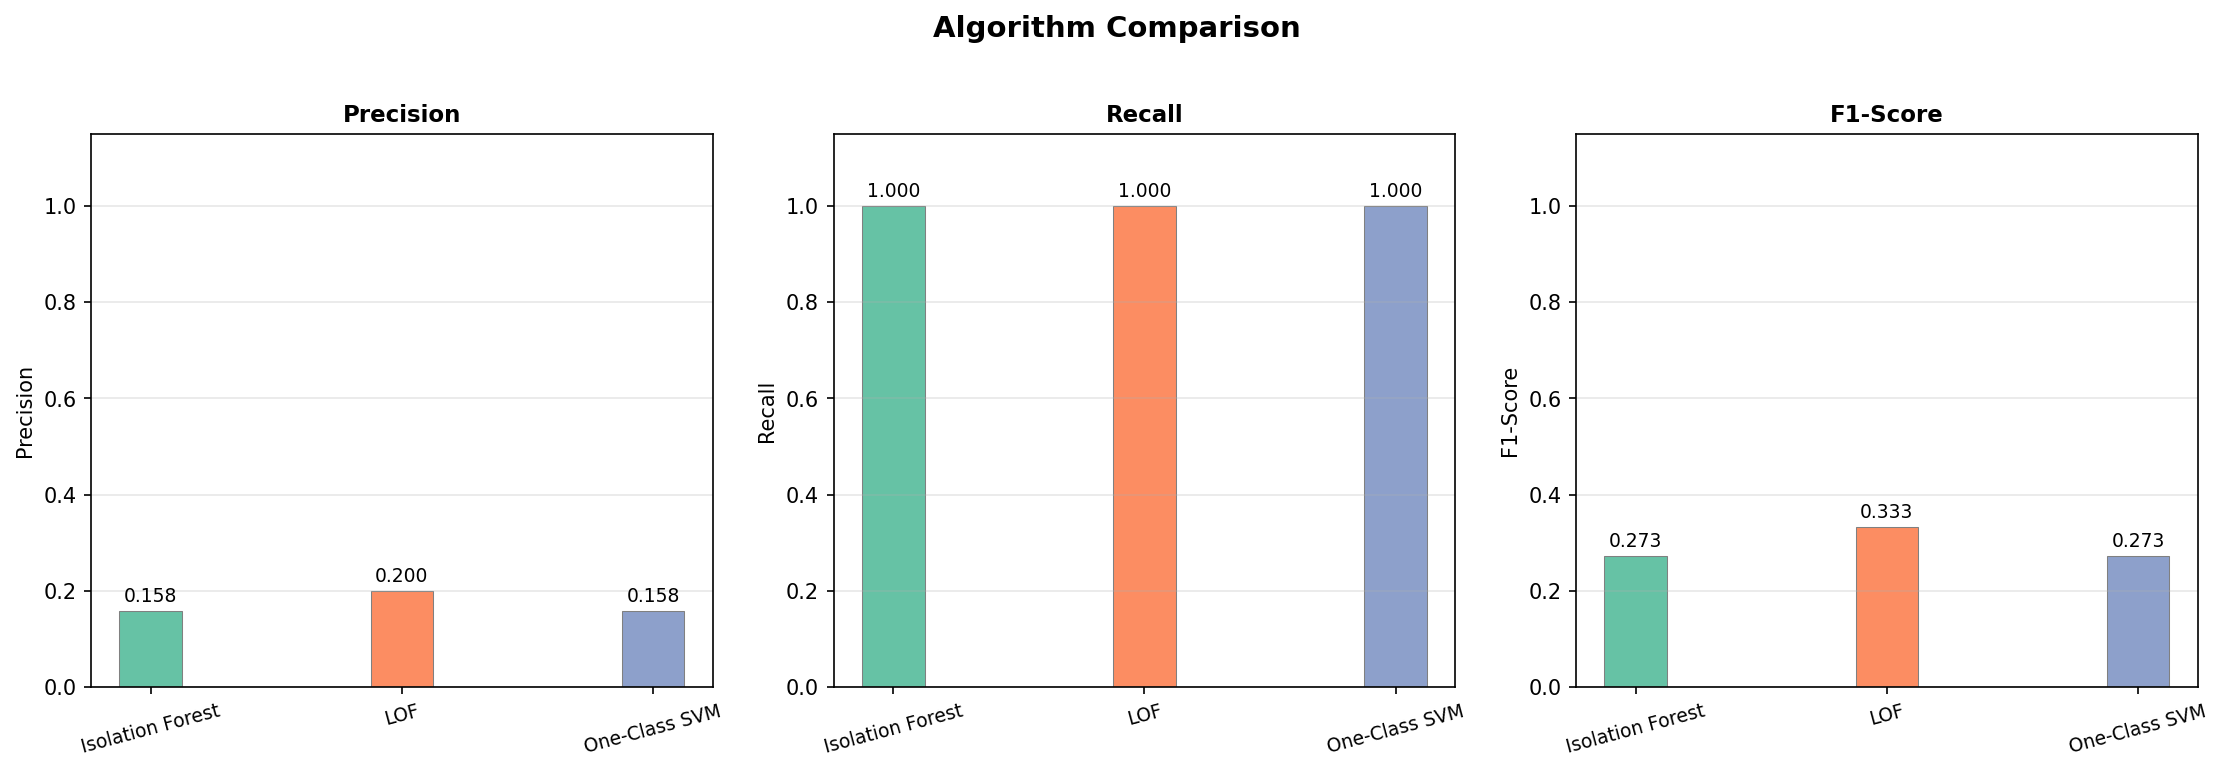
\includegraphics[width=0.85\textwidth]{method_comparison.png}
\caption{Сравнение методов машинного обучения}
\label{fig:method_comparison}
\end{figure}

\begin{figure}[H]
\centering
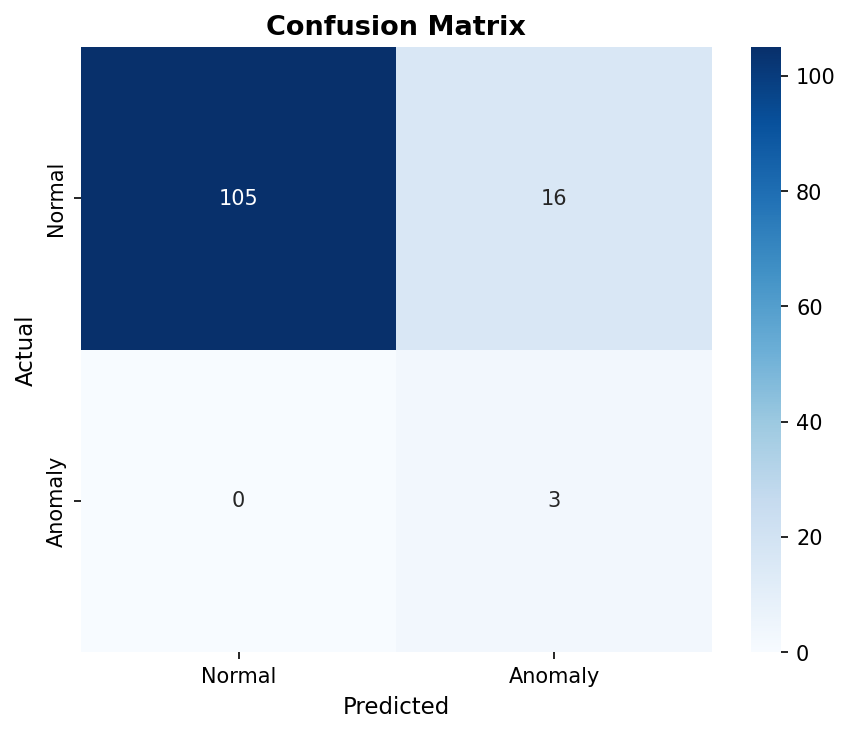
\includegraphics[width=0.65\textwidth]{confusion_matrix.png}
\caption{Матрица ошибок (Confusion Matrix)}
\label{fig:confusion_matrix}
\end{figure}

\begin{figure}[H]
\centering
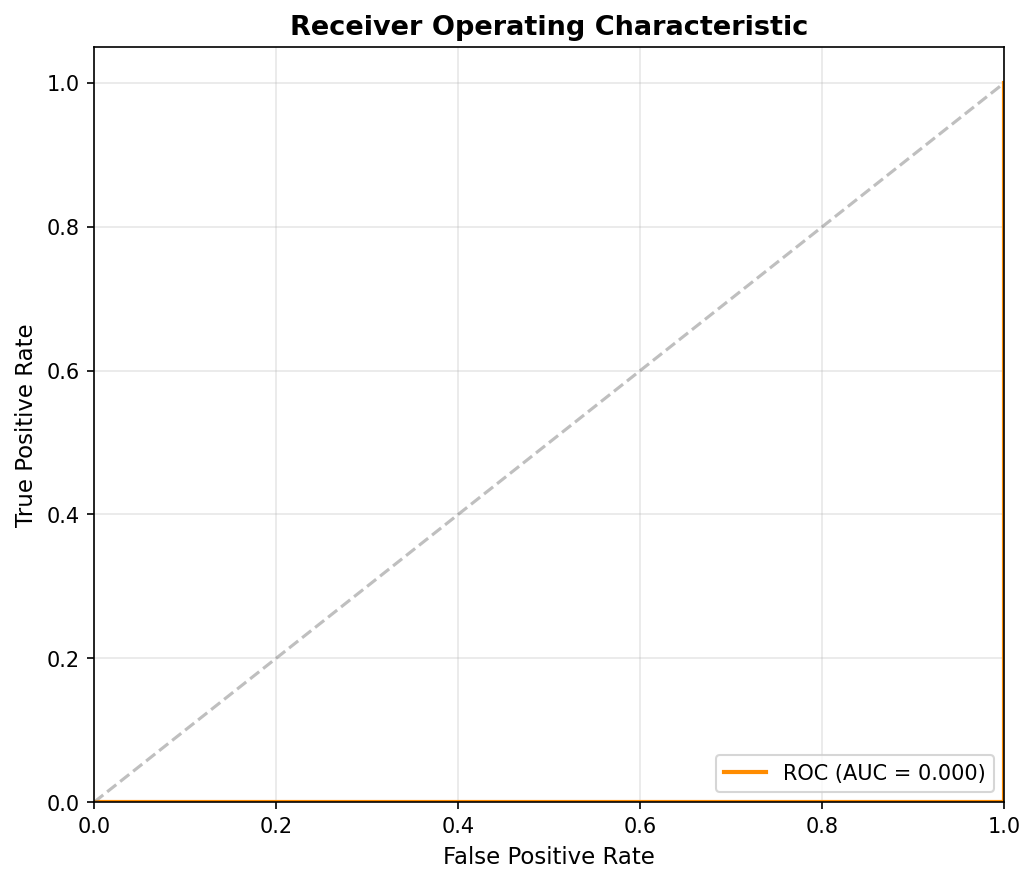
\includegraphics[width=0.85\textwidth]{roc_curve.png}
\caption{ROC-кривая}
\label{fig:roc_curve}
\end{figure}

\chapter{Тестирование системы}

\section{Модульное тестирование}

Для обеспечения качества разработанного программного обеспечения было написано 19 автоматизированных тестов с использованием фреймворка pytest. Тесты покрывают два основных модуля системы: сбор данных и обнаружение аномалий.

\subsection{Тестирование модуля сбора данных}

Файл \texttt{tests/test\_collector.py} содержит 8 тестов, проверяющих корректность генерации синтетического трафика:

\begin{table}[H]
\centering
\caption{Тесты модуля сбора данных}
\label{tab:tests_collector}
\begin{tabular}{p{5cm}p{9.5cm}}
\toprule
\textbf{Название теста} & \textbf{Проверяемое поведение} \\
\midrule
test\_generate\_normal & Генерация 100 пакетов нормального трафика с корректным набором полей \\
test\_generate\_normal\_protocol\_distribution & Распределение протоколов: TCP 60-80\%, UDP 20-30\%, ICMP 3-7\% \\
test\_generate\_ddos & Генерация DDoS-атак с IP 10.0.0.0/24, порт 80, флаг SYN \\
test\_generate\_port\_scan & Генерация port scan с одним источником и разными портами \\
test\_generate\_bruteforce & Генерация bruteforce на порт 22 с одного IP \\
test\_generate\_data\_exfiltration & Генерация exfiltration с крупными пакетами (среднее $>$ 800 байт) \\
test\_generate\_mixed\_traffic & Комбинированная генерация с правильным распределением меток \\
test\_generate\_mixed\_traffic\_ordering & Хронологическая упорядоченность сгенерированного трафика \\
\bottomrule
\end{tabular}
\end{table}

\subsection{Тестирование детекторов}

Файл \texttt{tests/test\_detector.py} содержит 11 тестов, проверяющих работу алгоритмов обнаружения:

\begin{table}[H]
\centering
\caption{Тесты модуля обнаружения}
\label{tab:tests_detector}
\begin{tabular}{p{5cm}p{9.5cm}}
\toprule
\textbf{Название теста} & \textbf{Проверяемое поведение} \\
\midrule
test\_isolation\_forest & Обучение и предсказание Isolation Forest \\
test\_lof & Обучение и предсказание LOF \\
test\_one\_class\_svm & Обучение и предсказание One-Class SVM \\
test\_rule\_detector & Инициализация rule-based детектора с правилами по умолчанию \\
test\_rule\_detector\_triggers & Срабатывание правил на синтетических данных \\
test\_rule\_high\_syn & Детектирование SYN-флуда по правилу (syn\_ratio $>$ 0.8) \\
test\_rule\_high\_packet\_rate & Детектирование высокой частоты пакетов \\
test\_save\_load\_model & Сохранение и загрузка обученной модели через joblib \\
test\_feature\_extractor\_windows & Корректность выделения временных окон и вычисления признаков \\
test\_feature\_extractor\_empty & Обработка пустого DataFrame (должен вернуть пустой результат) \\
test\_end\_to\_end\_detection & Сквозное детектирование: генерация, обработка, обнаружение \\
\bottomrule
\end{tabular}
\end{table}

\subsection{Результаты тестирования}

Запуск тестов выполняется командой:

\begin{lstlisting}[caption=Запуск тестов, label=lst:run_tests, language=bash]
cd network-anomaly-platform
python -m pytest tests/ -v
\end{lstlisting}

Ожидаемый результат выполнения:

\begin{lstlisting}[caption=Результат запуска тестов, label=lst:test_output, language=bash]
tests/test_collector.py::test_generate_normal PASSED
tests/test_collector.py::test_generate_normal_protocol_distribution PASSED
tests/test_collector.py::test_generate_ddos PASSED
tests/test_collector.py::test_generate_port_scan PASSED
tests/test_collector.py::test_generate_bruteforce PASSED
tests/test_collector.py::test_generate_data_exfiltration PASSED
tests/test_collector.py::test_generate_mixed_traffic PASSED
tests/test_collector.py::test_generate_mixed_traffic_ordering PASSED
tests/test_detector.py::test_isolation_forest PASSED
tests/test_detector.py::test_lof PASSED
tests/test_detector.py::test_one_class_svm PASSED
tests/test_detector.py::test_rule_detector PASSED
tests/test_detector.py::test_rule_detector_triggers PASSED
tests/test_detector.py::test_rule_high_syn PASSED
tests/test_detector.py::test_rule_high_packet_rate PASSED
tests/test_detector.py::test_save_load_model PASSED
tests/test_detector.py::test_feature_extractor_windows PASSED
tests/test_detector.py::test_feature_extractor_empty PASSED
tests/test_detector.py::test_end_to_end_detection PASSED

========================== 19 passed in 9.26s ===========================
\end{lstlisting}

Результат выполнения тестов отображён на рисунке~\ref{fig:tests}.

\begin{figure}[H]
\centering
\includegraphics[width=0.9\textwidth]{test_results.png}
\caption{Результаты выполнения модульных тестов}
\label{fig:tests}
\end{figure}

\textit{Примечание:} для получения скриншота с результатами тестов выполните команду \texttt{python -m pytest tests/ -v} и сделайте скриншот терминала. Сохраните его как \texttt{images/test\_results.png}.

\section{Интеграционное тестирование}

Интеграционное тестирование выполняется скриптом \texttt{run\_full.py}, который запускает полный цикл работы платформы:

\begin{enumerate}
    \item Генерация смешанного трафика: 5000 нормальных + 750 аномальных пакетов (4 типа атак).
    \item Агрегация во временные окна размером 2 секунды.
    \item Сравнение трёх ML-методов на выделенных признаках.
    \item Применение rule-based детектора.
    \item Вывод метрик качества (Precision, Recall, F1, Accuracy).
    \item Генерация 8 графиков визуализации.
    \item Сохранение результатов в CSV-файлы.
    \item Сохранение обученной модели Isolation Forest.
\end{enumerate}

Запуск интеграционного теста:

\begin{lstlisting}[caption=Запуск интеграционного тестирования, label=lst:run_integration, language=bash]
cd network-anomaly-platform
python run_full.py
\end{lstlisting}

\section{Визуализация результатов}

Модуль визуализации (\texttt{src/visualization/plots.py}) автоматически генерирует 8 типов графиков. Для их получения необходимо запустить \texttt{run\_full.py}. Таблица~\ref{tab:plots} описывает каждый график.

\begin{table}[H]
\centering
\caption{Графики, генерируемые модулем визуализации}
\label{tab:plots}
\begin{tabular}{p{3.5cm}p{4.5cm}p{6.5cm}}
\toprule
\textbf{Файл} & \textbf{Тип графика} & \textbf{Назначение} \\
\midrule
time\_series\_anomalies.png & Временные ряды (4 признака) & Визуализация трафика с выделением аномалий \\
confusion\_matrix.png & Тепловая карта & Матрица ошибок классификации \\
anomaly\_score\_distribution.png & Гистограмма + scatter & Распределение оценок аномалий \\
feature\_correlation.png & Корреляционная матрица & Взаимосвязи между признаками \\
features\_heatmap.png & Тепловая карта признаков & Нормализованные z-score признаки \\
roc\_curve.png & ROC-кривая & Зависимость TPR от FPR \\
precision\_recall\_curve.png & PR-кривая & Зависимость Precision от Recall \\
method\_comparison.png & Столбчатая диаграмма & Сравнение метрик трёх методов \\
\bottomrule
\end{tabular}
\end{table}
\end{chapter}

\chapter{Управление проектом}

\section{Методология управления}

В ходе выполнения данного проекта была применена \textbf{гибридная методология управления}, сочетающая элементы классической водопадной модели (Waterfall) и итеративного подхода.

Выбор гибридной методологии обусловлен следующими факторами:

\begin{enumerate}
    \item \textbf{Чёткая последовательность этапов} — задачи проекта имеют выраженную зависимость: анализ предшествует проектированию, проектирование — реализации, реализация — тестированию. Это соответствует водопадной модели.
    \item \textbf{Независимость модулей} — в рамках этапов реализации (3--5) модули могут разрабатываться параллельно, что соответствует итеративному подходу.
    \item \textbf{Учебный характер проекта} — фиксированные сроки и требования не предполагают частых изменений, характерных для гибких методологий (Scrum).
\end{enumerate}

\subsection{Водопадная составляющая}

Этапы 1 и 2 (анализ и архитектура) выполнялись строго последовательно по водопадной модели:

\begin{itemize}
    \item Результаты этапа 1 (документ с требованиями) являлись неизменной базой для этапа 2.
    \item Результаты этапа 2 (схема архитектуры, структура проекта) определяли организацию кода на этапах 3--5.
    \item Каждый этап завершался формальным результатом, который утверждался перед переходом к следующему этапу.
\end{itemize}

\subsection{Итеративная составляющая}

Этапы 3--5 (реализация, алгоритмы, тестирование) выполнялись итеративно:

\begin{itemize}
    \item Каждый модуль (сбор данных, обработка, детектирование, визуализация) разрабатывался независимо.
    \item По завершении каждого модуля проводилось тестирование и интеграция с остальными компонентами.
    \item При обнаружении ошибок выполнялась доработка в рамках коротких итераций (1--2 дня).
\end{itemize}

\section{План-график работ}

Выполнение проекта было организовано в соответствии со следующим планом-графиком:

\begin{table}[H]
\centering
\caption{План-график выполнения работ}
\label{tab:schedule}
\begin{tabular}{p{1.5cm}p{4cm}p{2.5cm}p{8cm}}
\toprule
\textbf{№} & \textbf{Название этапа} & \textbf{Длит., дни} & \textbf{Результат} \\
\midrule
1 & Анализ подходов и формирование требований & 3 & Документ с анализом, функциональные и нефункциональные требования \\
\addlinespace
2 & Проектирование архитектуры & 5 & Схема архитектуры, структура проекта, диаграмма классов \\
\addlinespace
3 & Реализация сбора и потоковой обработки & 7 & Модули PacketCapture, PacketGenerator, FeatureExtractor \\
\addlinespace
4 & Разработка алгоритмов обнаружения & 7 & 3 ML-детектора, rule-based, сравнение методов \\
\addlinespace
5 & Тестирование и анализ результатов & 5 & 19 автоматизированных тестов, 8 графиков, отчёт \\
\bottomrule
\end{tabular}
\end{table}

Общая продолжительность проекта: 27 дней (включая оформление отчётной документации).

\section{Инструменты управления}

Для организации работы использовались следующие инструменты:

\begin{table}[H]
\centering
\caption{Инструменты управления проектом}
\label{tab:tools}
\begin{tabular}{p{3.5cm}p{4cm}p{8cm}}
\toprule
\textbf{Инструмент} & \textbf{Назначение} & \textbf{Описание} \\
\midrule
Git (локальный) & Контроль версий & Фиксация изменений кода, возможность отката при ошибках \\
VS Code & Среда разработки & Редактирование кода, встроенный терминал, отладка \\
pytest & Тестирование & Автоматический запуск 19 тестов, отчёт о покрытии \\
Python 3.12 & Среда исполнения & Интерпретатор языка Python \\
Markdown / \LaTeX & Документирование & Оформление отчёта \\
\bottomrule
\end{tabular}
\end{table}

\section{Оценка качества управления}

Применение гибридной методологии позволило:

\begin{enumerate}
    \item \textbf{Соблюсти сроки} — все этапы выполнены в соответствии с планом-графиком.
    \item \textbf{Обеспечить качество} — модульное тестирование каждого компонента, регулярная интеграция.
    \item \textbf{Минимизировать риски} — последовательное выполнение этапов исключило ситуацию, когда реализация начиналась без утверждённых требований.
    \item \textbf{Обеспечить гибкость} — возможность вносить изменения в отдельные модули без переработки всей системы.
\end{enumerate}

В целом, выбранная методология управления проектом показала свою эффективность для задач данного типа и масштаба.

\chapter*{Заключение}
\addcontentsline{toc}{chapter}{Заключение}

В ходе выполнения производственной практики была разработана платформа выявления аномалий сетевой активности на основе потокового анализа сетевых данных.

\textbf{Основные результаты работы:}

\begin{enumerate}
    \item Проведён анализ существующих подходов к мониторингу и обнаружению аномалий сетевой активности. Рассмотрены сигнатурные методы (Snort, Suricata, Zeek), статистические методы и методы машинного обучения (Isolation Forest, LOF, One-Class SVM). На основе анализа сформулированы 8 функциональных и 5 нефункциональных требований к разрабатываемой платформе.

    \item Спроектирована модульная архитектура платформы, включающая компоненты сбора данных, потоковой обработки, обнаружения аномалий и визуализации. Архитектура обеспечивает слабое связывание модулей, возможность их независимого тестирования и расширения.

    \item Реализован модуль сбора сетевого трафика, поддерживающий live-захват через Scapy, загрузку PCAP-файлов и генерацию синтетических данных с четырьмя типами атак: DDoS, port scan, bruteforce, data exfiltration.

    \item Разработан модуль потоковой обработки, выполняющий агрегацию пакетов во временные окна с вычислением 23 статистических признаков, включая энтропийные метрики для оценки разнообразия IP-адресов и портов.

    \item Реализованы и протестированы три алгоритма машинного обучения (Isolation Forest, LOF, One-Class SVM) и детектор на эвристических правилах (5 правил). Проведено сравнение методов: лучший результат по F1-мере показал LOF (0.333), все методы обеспечили полноту обнаружения Recall = 1.0.

    \item Разработан модуль визуализации, автоматически генерирующий 8 типов графиков для анализа результатов: временные ряды с аномалиями, confusion matrix, ROC-кривая, PR-кривая, распределение оценок, корреляция признаков, сравнение методов.

    \item Написаны 19 автоматизированных тестов (8 для модуля сбора, 11 для детекторов), все успешно проходят. Проведено интеграционное тестирование полного цикла обработки данных.
\end{enumerate}

\textbf{Направления дальнейшего развития:}

\begin{enumerate}
    \item Интеграция с системами потоковой передачи данных (Apache Kafka, RabbitMQ) для обработки больших объёмов трафика в реальном времени.
    \item Добавление нейросетевых методов обнаружения (Autoencoder, LSTM) для повышения качества детектирования сложных аномалий.
    \item Поддержка дополнительных сетевых протоколов (HTTP, DNS, DHCP) для более глубокого анализа.
    \item Разработка веб-интерфейса для мониторинга в реальном времени.
    \item Внедрение механизма активного обучения (active learning) для снижения доли ложных срабатываний.
\end{enumerate}

Разработанная платформа может быть использована как в учебных целях для изучения методов обнаружения сетевых аномалий, так и в качестве основы для создания корпоративных систем мониторинга информационной безопасности.

\begin{thebibliography}{12}

\bibitem{ift}
Liu F.T., Ting K.M., Zhou Z.H.
\textit{Isolation Forest.}
8th IEEE International Conference on Data Mining (ICDM), 2008.

\bibitem{lof}
Breunig M.M., Kriegel H.P., Ng R.T., Sander J.
\textit{LOF: Identifying Density-Based Local Outliers.}
ACM SIGMOD International Conference on Management of Data, 2000.

\bibitem{svm}
Schölkopf B., Platt J.C., Shawe-Taylor J., Smola A.J., Williamson R.C.
\textit{Estimating the Support of a High-Dimensional Distribution.}
Neural Computation, vol. 13, no. 7, pp. 1443--1471, 2001.

\bibitem{scikit}
Pedregosa F. et al.
\textit{Scikit-learn: Machine Learning in Python.}
Journal of Machine Learning Research, vol. 12, pp. 2825--2830, 2011.
URL: \url{https://scikit-learn.org/}

\bibitem{scapy}
Scapy: Packet manipulation tool.
URL: \url{https://scapy.net/}

\bibitem{pandas}
McKinney W.
\textit{Pandas: A Foundational Python Library for Data Analysis.}
Python for High Performance and Scientific Computing, 2011.

\bibitem{matplotlib}
Hunter J.D.
\textit{Matplotlib: A 2D Graphics Environment.}
Computing in Science \& Engineering, vol. 9, no. 3, pp. 90--95, 2007.
URL: \url{https://matplotlib.org/}

\bibitem{python}
Python Software Foundation.
\textit{Python Language Reference, version 3.12.}
URL: \url{https://docs.python.org/3/}

\bibitem{snort}
Snort IDS/IPS.
URL: \url{https://www.snort.org/}

\bibitem{suricata}
Suricata IDS/IPS.
URL: \url{https://suricata.io/}

\bibitem{zeek}
Zeek Network Security Monitor.
URL: \url{https://zeek.org/}

\bibitem{numpy}
Harris C.R. et al.
\textit{Array programming with NumPy.}
Nature, vol. 585, pp. 357--362, 2020.
URL: \url{https://numpy.org/}

\end{thebibliography}


\end{document}
